\documentclass[twoside]{book}

% Packages required by doxygen
\usepackage{fixltx2e}
\usepackage{calc}
\usepackage{doxygen}
\usepackage[export]{adjustbox} % also loads graphicx
\usepackage{graphicx}
\usepackage[utf8]{inputenc}
\usepackage{makeidx}
\usepackage{multicol}
\usepackage{multirow}
\PassOptionsToPackage{warn}{textcomp}
\usepackage{textcomp}
\usepackage[nointegrals]{wasysym}
\usepackage[table]{xcolor}

% Font selection
\usepackage[T1]{fontenc}
\usepackage[scaled=.90]{helvet}
\usepackage{courier}
\usepackage{amssymb}
\usepackage{sectsty}
\renewcommand{\familydefault}{\sfdefault}
\allsectionsfont{%
  \fontseries{bc}\selectfont%
  \color{darkgray}%
}
\renewcommand{\DoxyLabelFont}{%
  \fontseries{bc}\selectfont%
  \color{darkgray}%
}
\newcommand{\+}{\discretionary{\mbox{\scriptsize$\hookleftarrow$}}{}{}}

% Page & text layout
\usepackage{geometry}
\geometry{%
  a4paper,%
  top=2.5cm,%
  bottom=2.5cm,%
  left=2.5cm,%
  right=2.5cm%
}
\tolerance=750
\hfuzz=15pt
\hbadness=750
\setlength{\emergencystretch}{15pt}
\setlength{\parindent}{0cm}
\setlength{\parskip}{3ex plus 2ex minus 2ex}
\makeatletter
\renewcommand{\paragraph}{%
  \@startsection{paragraph}{4}{0ex}{-1.0ex}{1.0ex}{%
    \normalfont\normalsize\bfseries\SS@parafont%
  }%
}
\renewcommand{\subparagraph}{%
  \@startsection{subparagraph}{5}{0ex}{-1.0ex}{1.0ex}{%
    \normalfont\normalsize\bfseries\SS@subparafont%
  }%
}
\makeatother

% Headers & footers
\usepackage{fancyhdr}
\pagestyle{fancyplain}
\fancyhead[LE]{\fancyplain{}{\bfseries\thepage}}
\fancyhead[CE]{\fancyplain{}{}}
\fancyhead[RE]{\fancyplain{}{\bfseries\leftmark}}
\fancyhead[LO]{\fancyplain{}{\bfseries\rightmark}}
\fancyhead[CO]{\fancyplain{}{}}
\fancyhead[RO]{\fancyplain{}{\bfseries\thepage}}
\fancyfoot[LE]{\fancyplain{}{}}
\fancyfoot[CE]{\fancyplain{}{}}
\fancyfoot[RE]{\fancyplain{}{\bfseries\scriptsize Generated by Doxygen }}
\fancyfoot[LO]{\fancyplain{}{\bfseries\scriptsize Generated by Doxygen }}
\fancyfoot[CO]{\fancyplain{}{}}
\fancyfoot[RO]{\fancyplain{}{}}
\renewcommand{\footrulewidth}{0.4pt}
\renewcommand{\chaptermark}[1]{%
  \markboth{#1}{}%
}
\renewcommand{\sectionmark}[1]{%
  \markright{\thesection\ #1}%
}

% Indices & bibliography
\usepackage{natbib}
\usepackage[titles]{tocloft}
\setcounter{tocdepth}{3}
\setcounter{secnumdepth}{5}
\makeindex

% Hyperlinks (required, but should be loaded last)
\usepackage{ifpdf}
\ifpdf
  \usepackage[pdftex,pagebackref=true]{hyperref}
\else
  \usepackage[ps2pdf,pagebackref=true]{hyperref}
\fi
\hypersetup{%
  colorlinks=true,%
  linkcolor=blue,%
  citecolor=blue,%
  unicode%
}

% Custom commands
\newcommand{\clearemptydoublepage}{%
  \newpage{\pagestyle{empty}\cleardoublepage}%
}

\usepackage{caption}
\captionsetup{labelsep=space,justification=centering,font={bf},singlelinecheck=off,skip=4pt,position=top}

%===== C O N T E N T S =====

\begin{document}

% Titlepage & ToC
\hypersetup{pageanchor=false,
             bookmarksnumbered=true,
             pdfencoding=unicode
            }
\pagenumbering{alph}
\begin{titlepage}
\vspace*{7cm}
\begin{center}%
{\Large Gaussian Processes }\\
\vspace*{1cm}
{\large Generated by Doxygen 1.8.12}\\
\end{center}
\end{titlepage}
\clearemptydoublepage
\pagenumbering{roman}
\tableofcontents
\clearemptydoublepage
\pagenumbering{arabic}
\hypersetup{pageanchor=true}

%--- Begin generated contents ---
\chapter{Gaussian Processes}
\label{index}\hypertarget{index}{}\href{https://travis-ci.org/dfridovi/gp}{\tt } \href{https://github.com/dfridovi/gp/blob/master/LICENSE}{\tt }

A homebrewed C++ library for Gaussian processes. {\bfseries gp} is developed by \href{http://people.eecs.berkeley.edu/~dfk/}{\tt David Fridovich-\/\+Keil}, a second-\/year PhD student in the Berkeley \href{http://hybrid.eecs.berkeley.edu}{\tt Hybrid Systems Lab} and the \href{http://bair.berkeley.edu}{\tt Berkeley Artificial Intelligence Research (B\+A\+IR) Lab}.

\subsection*{Status}

{\bfseries gp} is still under active development. I hope to have a first release soon though, so stay tuned!

\subsection*{Structure}

All source code is located in {\ttfamily src/}; headers are in {\ttfamily include/}; unit tests are in {\ttfamily /test/}; and executables are in {\ttfamily exec/}. Compiled binaries will be placed in {\ttfamily bin/}.

\subsection*{Dependencies}

I may miss a few here, but here is a list of dependencies\+:


\begin{DoxyItemize}
\item \href{http://eigen.tuxfamily.org/dox/}{\tt Eigen} (header-\/only linear algebra library)
\item Gflags (Google\textquotesingle{}s command-\/line flag manager)
\item Glog (Google\textquotesingle{}s logging tool)
\end{DoxyItemize}

All of these may be installed very easily. If you run into any trouble, though, I am more than happy to help you figure out what\textquotesingle{}s going on. Just post an \href{https://github.com/dfridovi/gp/issues}{\tt issue} on this repository and I will reply as soon as possible.

\subsection*{Usage}

You\textquotesingle{}ll need to begin by building the repository. From the top directory, type the following sequence of commands\+:


\begin{DoxyCode}
mkdir bin
mkdir build
cd build
cmake ..
make -j4
\end{DoxyCode}


This should build all tests and executables. In order to run tests, you can run the following command\+:


\begin{DoxyCode}
./run\_tests
\end{DoxyCode}


from within the {\ttfamily build/} directory you just made. All the tests should pass, and none should take more than a second or so to run.

Executables are automatically placed within the {\ttfamily bin/} directory that you created. To run them, just type {\ttfamily ./(name-\/of-\/executable)}.

To the extent that it makes sense, all parameters are accessible from the command line via Gflags. For help with command line options, simply run the following command\+:


\begin{DoxyCode}
./(name-of-executable) --help
\end{DoxyCode}


\subsection*{A\+PI documentation}

I\textquotesingle{}ve been using Doxygen to auto-\/generate web-\/based \href{https://dfridovi.github.io/gp/documentation/html/}{\tt documentation}. Although I do not follow the Doxygen guidelines for writing comments, auto-\/generation still seems to do a fairly reasonable job. 
\chapter{Hierarchical Index}
\section{Class Hierarchy}
This inheritance list is sorted roughly, but not completely, alphabetically\+:\begin{DoxyCompactList}
\item First\+Order\+Function\begin{DoxyCompactList}
\item \contentsline{section}{gp\+:\+:Training\+Log\+Likelihood}{\pageref{classgp_1_1_training_log_likelihood}}{}
\end{DoxyCompactList}
\item \contentsline{section}{gp\+:\+:Gaussian\+Process}{\pageref{classgp_1_1_gaussian_process}}{}
\item \contentsline{section}{gp\+:\+:Kernel}{\pageref{classgp_1_1_kernel}}{}
\begin{DoxyCompactList}
\item \contentsline{section}{gp\+:\+:Rbf\+Kernel}{\pageref{classgp_1_1_rbf_kernel}}{}
\end{DoxyCompactList}
\item Mat\+Plot\begin{DoxyCompactList}
\item \contentsline{section}{gp\+:\+:Plot1D}{\pageref{classgp_1_1_plot1_d}}{}
\end{DoxyCompactList}
\end{DoxyCompactList}

\chapter{Class Index}
\section{Class List}
Here are the classes, structs, unions and interfaces with brief descriptions\+:\begin{DoxyCompactList}
\item\contentsline{section}{\hyperlink{classgp_1_1_gaussian_process}{gp\+::\+Gaussian\+Process} }{\pageref{classgp_1_1_gaussian_process}}{}
\item\contentsline{section}{\hyperlink{classgp_1_1_kernel}{gp\+::\+Kernel} }{\pageref{classgp_1_1_kernel}}{}
\item\contentsline{section}{\hyperlink{classgp_1_1_plot1_d}{gp\+::\+Plot1D} }{\pageref{classgp_1_1_plot1_d}}{}
\item\contentsline{section}{\hyperlink{classgp_1_1_rbf_kernel}{gp\+::\+Rbf\+Kernel} }{\pageref{classgp_1_1_rbf_kernel}}{}
\item\contentsline{section}{\hyperlink{classgp_1_1_training_log_likelihood}{gp\+::\+Training\+Log\+Likelihood} }{\pageref{classgp_1_1_training_log_likelihood}}{}
\end{DoxyCompactList}

\chapter{Class Documentation}
\hypertarget{classgp_1_1_gaussian_process}{}\section{gp\+:\+:Gaussian\+Process Class Reference}
\label{classgp_1_1_gaussian_process}\index{gp\+::\+Gaussian\+Process@{gp\+::\+Gaussian\+Process}}
\subsection*{Public Member Functions}
\begin{DoxyCompactItemize}
\item 
\hypertarget{classgp_1_1_gaussian_process_a47cdf94a91858d0931115260e5e1704c}{}\label{classgp_1_1_gaussian_process_a47cdf94a91858d0931115260e5e1704c} 
{\bfseries Gaussian\+Process} (const Kernel\+::\+Ptr \&kernel, double noise, size\+\_\+t dimension, size\+\_\+t max\+\_\+points=100)
\item 
\hypertarget{classgp_1_1_gaussian_process_a1e5a8059688294936f4396a88082e335}{}\label{classgp_1_1_gaussian_process_a1e5a8059688294936f4396a88082e335} 
{\bfseries Gaussian\+Process} (const Kernel\+::\+Ptr \&kernel, double noise, const Point\+Set \&points, size\+\_\+t max\+\_\+points=100)
\item 
\hypertarget{classgp_1_1_gaussian_process_a3dcd374d4090be21c059ef8ccde1519c}{}\label{classgp_1_1_gaussian_process_a3dcd374d4090be21c059ef8ccde1519c} 
{\bfseries Gaussian\+Process} (const Kernel\+::\+Ptr \&kernel, double noise, const Point\+Set \&points, const Vector\+Xd \&targets, size\+\_\+t max\+\_\+points=100)
\item 
\hypertarget{classgp_1_1_gaussian_process_a850493ba48793ad4bf2e17043d469928}{}\label{classgp_1_1_gaussian_process_a850493ba48793ad4bf2e17043d469928} 
void {\bfseries Evaluate} (const Vector\+Xd \&x, double \&mean, double \&variance) const
\item 
\hypertarget{classgp_1_1_gaussian_process_a2594af50120c38f7c3d4dd894fb07d32}{}\label{classgp_1_1_gaussian_process_a2594af50120c38f7c3d4dd894fb07d32} 
void {\bfseries Evaluate\+Training\+Point} (size\+\_\+t ii, double \&mean, double \&variance) const
\item 
\hypertarget{classgp_1_1_gaussian_process_a8ad3e9ac5a536ed71be83fac8ca4f0af}{}\label{classgp_1_1_gaussian_process_a8ad3e9ac5a536ed71be83fac8ca4f0af} 
bool {\bfseries Learn\+Hyperparams} ()
\item 
\hypertarget{classgp_1_1_gaussian_process_a4f55d908c1033b8d02f986321abc4257}{}\label{classgp_1_1_gaussian_process_a4f55d908c1033b8d02f986321abc4257} 
const Matrix\+Xd \& {\bfseries Immutable\+Covariance} () const
\item 
\hypertarget{classgp_1_1_gaussian_process_ac80689ba379920754defa7e585cf20bf}{}\label{classgp_1_1_gaussian_process_ac80689ba379920754defa7e585cf20bf} 
const Vector\+Xd \& {\bfseries Immutable\+Regressed\+Targets} () const
\item 
\hypertarget{classgp_1_1_gaussian_process_a281b5c08bb7a012203a49d992098e0c3}{}\label{classgp_1_1_gaussian_process_a281b5c08bb7a012203a49d992098e0c3} 
const Eigen\+::\+L\+LT$<$ Matrix\+Xd $>$ \& {\bfseries Immutable\+Cholesky} () const
\item 
\hypertarget{classgp_1_1_gaussian_process_ac1c7728df9a864da192ad77656f5567e}{}\label{classgp_1_1_gaussian_process_ac1c7728df9a864da192ad77656f5567e} 
size\+\_\+t {\bfseries Dimension} () const
\end{DoxyCompactItemize}


\subsection{Detailed Description}


Definition at line 55 of file gaussian\+\_\+process.\+hpp.



The documentation for this class was generated from the following files\+:\begin{DoxyCompactItemize}
\item 
/\+Users/davidfridovichkeil/\+Documents/\+Developer/gp/include/process/gaussian\+\_\+process.\+hpp\item 
/\+Users/davidfridovichkeil/\+Documents/\+Developer/gp/src/process/gaussian\+\_\+process.\+cpp\end{DoxyCompactItemize}

\hypertarget{classgp_1_1_kernel}{}\section{gp\+:\+:Kernel Class Reference}
\label{classgp_1_1_kernel}\index{gp\+::\+Kernel@{gp\+::\+Kernel}}
Inheritance diagram for gp\+:\+:Kernel\+:\begin{figure}[H]
\begin{center}
\leavevmode
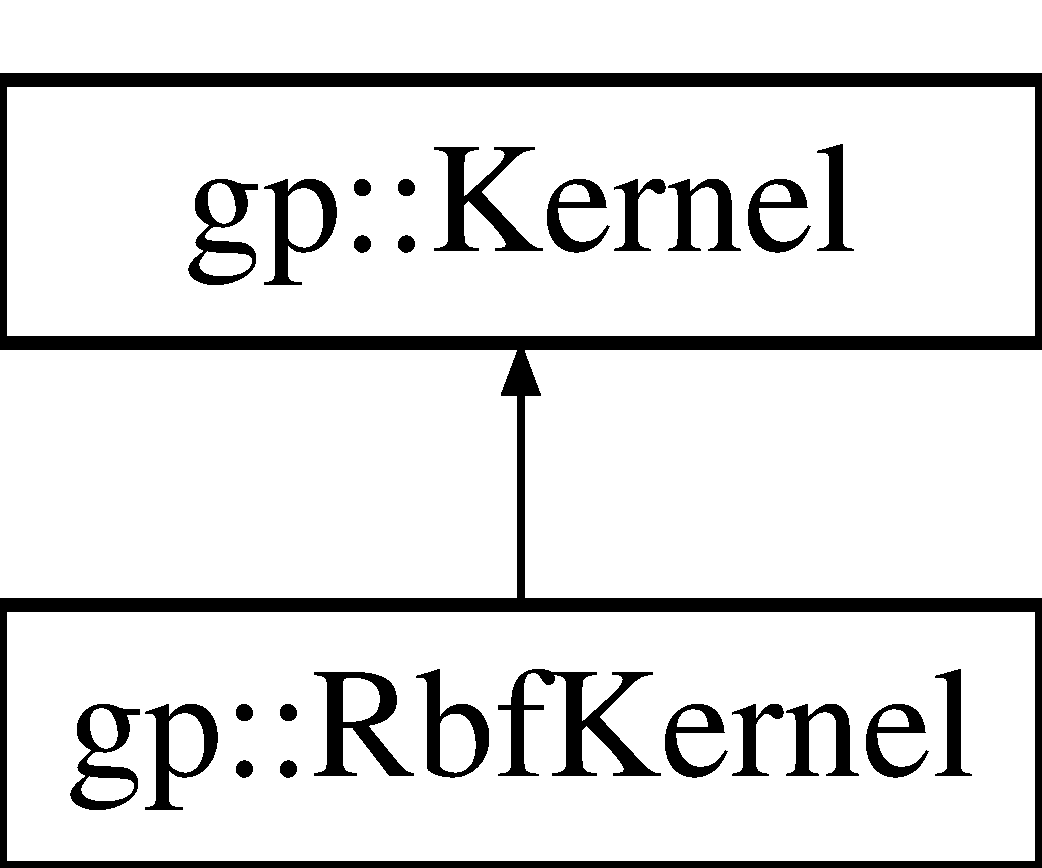
\includegraphics[height=2.000000cm]{classgp_1_1_kernel}
\end{center}
\end{figure}
\subsection*{Public Types}
\begin{DoxyCompactItemize}
\item 
\hypertarget{classgp_1_1_kernel_a8029bbf70cbb1af8c54ef1fe5c180880}{}\label{classgp_1_1_kernel_a8029bbf70cbb1af8c54ef1fe5c180880} 
typedef std\+::shared\+\_\+ptr$<$ \hyperlink{classgp_1_1_kernel}{Kernel} $>$ {\bfseries Ptr}
\item 
\hypertarget{classgp_1_1_kernel_a6aad36652792684a96ee86b704697139}{}\label{classgp_1_1_kernel_a6aad36652792684a96ee86b704697139} 
typedef std\+::shared\+\_\+ptr$<$ const \hyperlink{classgp_1_1_kernel}{Kernel} $>$ {\bfseries Const\+Ptr}
\end{DoxyCompactItemize}
\subsection*{Public Member Functions}
\begin{DoxyCompactItemize}
\item 
\hypertarget{classgp_1_1_kernel_aa9918f8604f04d60b34a63af9cb266ff}{}\label{classgp_1_1_kernel_aa9918f8604f04d60b34a63af9cb266ff} 
virtual double {\bfseries Evaluate} (const Vector\+Xd \&x, const Vector\+Xd \&y) const =0
\item 
\hypertarget{classgp_1_1_kernel_ab24d8d0274352f66775a945200a0c890}{}\label{classgp_1_1_kernel_ab24d8d0274352f66775a945200a0c890} 
virtual double {\bfseries Partial} (const Vector\+Xd \&x, const Vector\+Xd \&y, size\+\_\+t ii) const =0
\item 
\hypertarget{classgp_1_1_kernel_a6c295cdaae3faa53c57a116256c9a563}{}\label{classgp_1_1_kernel_a6c295cdaae3faa53c57a116256c9a563} 
virtual void {\bfseries Gradient} (const Vector\+Xd \&x, const Vector\+Xd \&y, Vector\+Xd \&gradient) const =0
\item 
\hypertarget{classgp_1_1_kernel_a50cc0098ee88720b46a6b42b854bd238}{}\label{classgp_1_1_kernel_a50cc0098ee88720b46a6b42b854bd238} 
Vector\+Xd \& {\bfseries Params} ()
\item 
\hypertarget{classgp_1_1_kernel_a9afcb83dbab5e1fbc6f8cb58af3c744d}{}\label{classgp_1_1_kernel_a9afcb83dbab5e1fbc6f8cb58af3c744d} 
const Vector\+Xd \& {\bfseries Immutable\+Params} () const
\item 
\hypertarget{classgp_1_1_kernel_a1f98048676af7164184cd23e53aa64cc}{}\label{classgp_1_1_kernel_a1f98048676af7164184cd23e53aa64cc} 
void {\bfseries Reset} (const Vector\+Xd \&params)
\item 
\hypertarget{classgp_1_1_kernel_a24217ef59b1a7da0c930e0969909680b}{}\label{classgp_1_1_kernel_a24217ef59b1a7da0c930e0969909680b} 
void {\bfseries Adjust} (double diff, size\+\_\+t ii)
\end{DoxyCompactItemize}
\subsection*{Protected Member Functions}
\begin{DoxyCompactItemize}
\item 
\hypertarget{classgp_1_1_kernel_a4faf4a711b0d6c88b10643c50f251103}{}\label{classgp_1_1_kernel_a4faf4a711b0d6c88b10643c50f251103} 
{\bfseries Kernel} (const Vector\+Xd \&params)
\end{DoxyCompactItemize}
\subsection*{Protected Attributes}
\begin{DoxyCompactItemize}
\item 
\hypertarget{classgp_1_1_kernel_af79e9cbee5be105a6e9393e2f6fba5db}{}\label{classgp_1_1_kernel_af79e9cbee5be105a6e9393e2f6fba5db} 
Vector\+Xd {\bfseries params\+\_\+}
\end{DoxyCompactItemize}


\subsection{Detailed Description}


Definition at line 55 of file kernel.\+hpp.



The documentation for this class was generated from the following file\+:\begin{DoxyCompactItemize}
\item 
/\+Users/davidfridovichkeil/\+Documents/\+Developer/gp/include/kernels/kernel.\+hpp\end{DoxyCompactItemize}

\hypertarget{classgp_1_1_plot1_d}{}\section{gp\+:\+:Plot1D Class Reference}
\label{classgp_1_1_plot1_d}\index{gp\+::\+Plot1D@{gp\+::\+Plot1D}}
Inheritance diagram for gp\+:\+:Plot1D\+:\begin{figure}[H]
\begin{center}
\leavevmode
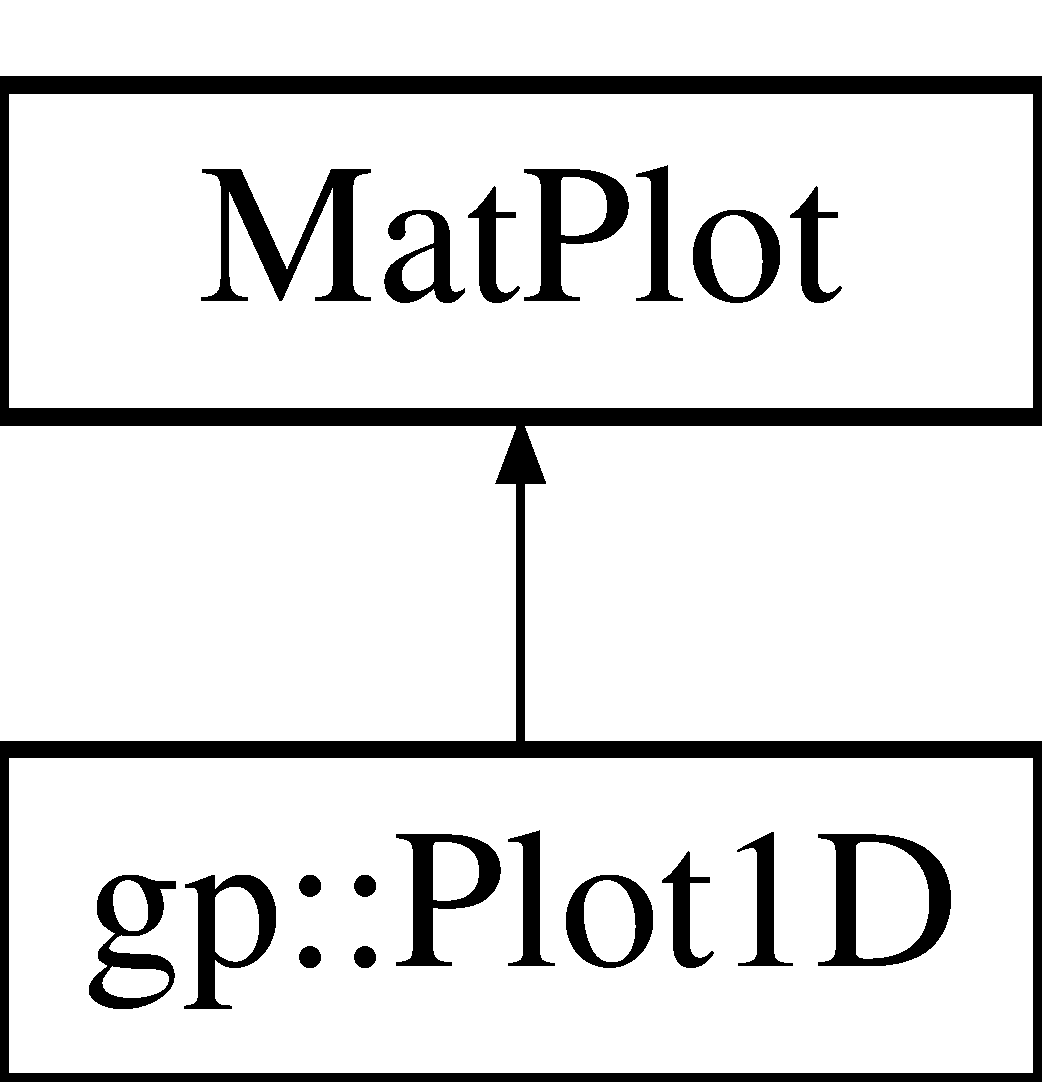
\includegraphics[height=2.000000cm]{classgp_1_1_plot1_d}
\end{center}
\end{figure}
\subsection*{Public Member Functions}
\begin{DoxyCompactItemize}
\item 
\hypertarget{classgp_1_1_plot1_d_a1f37c38e062adebdfad1c8e3f242109e}{}\label{classgp_1_1_plot1_d_a1f37c38e062adebdfad1c8e3f242109e} 
{\bfseries Plot1D} (const \hyperlink{classgp_1_1_gaussian_process}{Gaussian\+Process} $\ast$const gp, double xmin, double xmax, double ymin, double ymax, size\+\_\+t num\+\_\+points=100, const std\+::string \&title=\char`\"{}\char`\"{}, const std\+::string \&xlabel=\char`\"{}\char`\"{}, const std\+::string \&ylabel=\char`\"{}\char`\"{})
\item 
\hypertarget{classgp_1_1_plot1_d_a63c88cd7b1231277a0f19208516f07dd}{}\label{classgp_1_1_plot1_d_a63c88cd7b1231277a0f19208516f07dd} 
void {\bfseries D\+I\+S\+P\+L\+AY} ()
\end{DoxyCompactItemize}


\subsection{Detailed Description}


Definition at line 55 of file plot\+\_\+1d.\+hpp.



The documentation for this class was generated from the following file\+:\begin{DoxyCompactItemize}
\item 
/\+Users/davidfridovichkeil/\+Documents/\+Developer/gp/include/utils/plot\+\_\+1d.\+hpp\end{DoxyCompactItemize}

\hypertarget{classgp_1_1_rbf_kernel}{}\section{gp\+:\+:Rbf\+Kernel Class Reference}
\label{classgp_1_1_rbf_kernel}\index{gp\+::\+Rbf\+Kernel@{gp\+::\+Rbf\+Kernel}}
Inheritance diagram for gp\+:\+:Rbf\+Kernel\+:\begin{figure}[H]
\begin{center}
\leavevmode
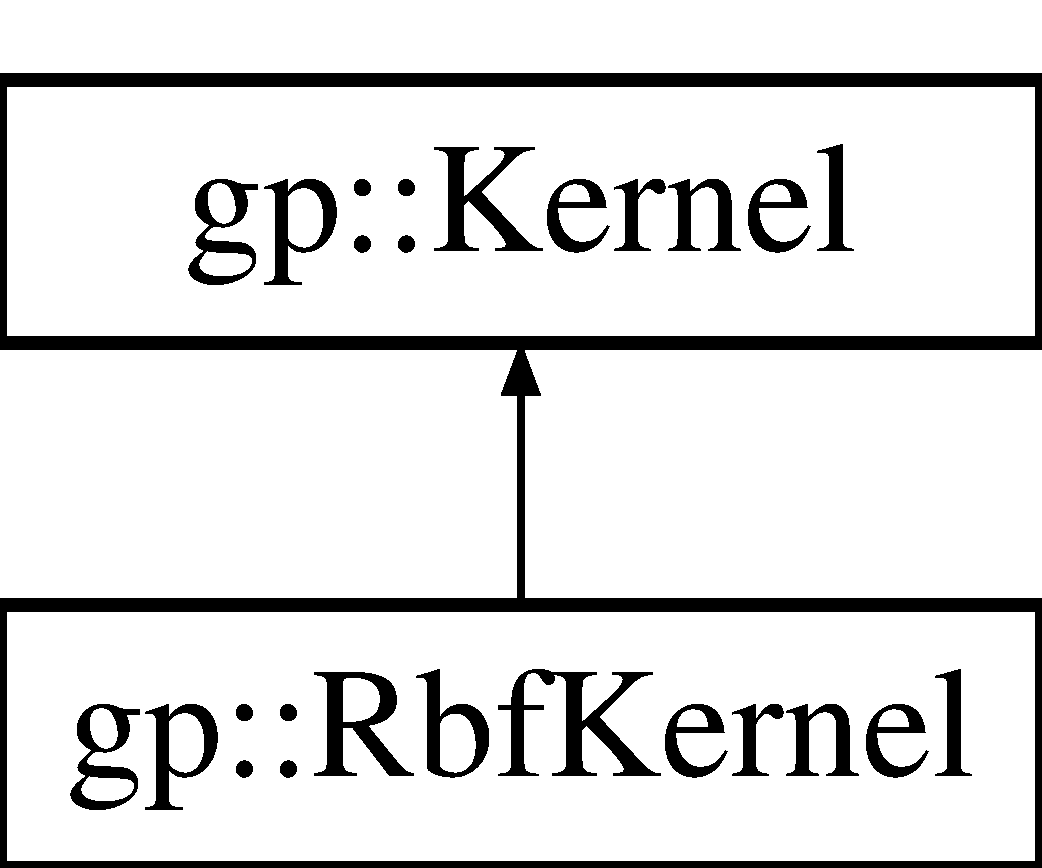
\includegraphics[height=2.000000cm]{classgp_1_1_rbf_kernel}
\end{center}
\end{figure}
\subsection*{Public Member Functions}
\begin{DoxyCompactItemize}
\item 
\hypertarget{classgp_1_1_rbf_kernel_a580c375d8dc6850991b68bdc7a73f426}{}\label{classgp_1_1_rbf_kernel_a580c375d8dc6850991b68bdc7a73f426} 
double {\bfseries Evaluate} (const Vector\+Xd \&x, const Vector\+Xd \&y) const
\item 
\hypertarget{classgp_1_1_rbf_kernel_a6b547d97211b02629ac4b19344c0c3f7}{}\label{classgp_1_1_rbf_kernel_a6b547d97211b02629ac4b19344c0c3f7} 
double {\bfseries Partial} (const Vector\+Xd \&x, const Vector\+Xd \&y, size\+\_\+t ii) const
\item 
\hypertarget{classgp_1_1_rbf_kernel_a54f8f958a7fe109fcd39fb1ea43fa5a0}{}\label{classgp_1_1_rbf_kernel_a54f8f958a7fe109fcd39fb1ea43fa5a0} 
void {\bfseries Gradient} (const Vector\+Xd \&x, const Vector\+Xd \&y, Vector\+Xd \&gradient) const
\end{DoxyCompactItemize}
\subsection*{Static Public Member Functions}
\begin{DoxyCompactItemize}
\item 
\hypertarget{classgp_1_1_rbf_kernel_a9576aa74cfd78fb43d671e748cc7cf49}{}\label{classgp_1_1_rbf_kernel_a9576aa74cfd78fb43d671e748cc7cf49} 
static Kernel\+::\+Ptr {\bfseries Create} (const Vector\+Xd \&lengths)
\end{DoxyCompactItemize}
\subsection*{Additional Inherited Members}


\subsection{Detailed Description}


Definition at line 52 of file rbf\+\_\+kernel.\+hpp.



The documentation for this class was generated from the following files\+:\begin{DoxyCompactItemize}
\item 
/\+Users/davidfridovichkeil/\+Documents/\+Developer/gp/include/kernels/rbf\+\_\+kernel.\+hpp\item 
/\+Users/davidfridovichkeil/\+Documents/\+Developer/gp/src/kernels/rbf\+\_\+kernel.\+cpp\end{DoxyCompactItemize}

\hypertarget{classgp_1_1_training_log_likelihood}{}\section{gp\+:\+:Training\+Log\+Likelihood Class Reference}
\label{classgp_1_1_training_log_likelihood}\index{gp\+::\+Training\+Log\+Likelihood@{gp\+::\+Training\+Log\+Likelihood}}
Inheritance diagram for gp\+:\+:Training\+Log\+Likelihood\+:\begin{figure}[H]
\begin{center}
\leavevmode
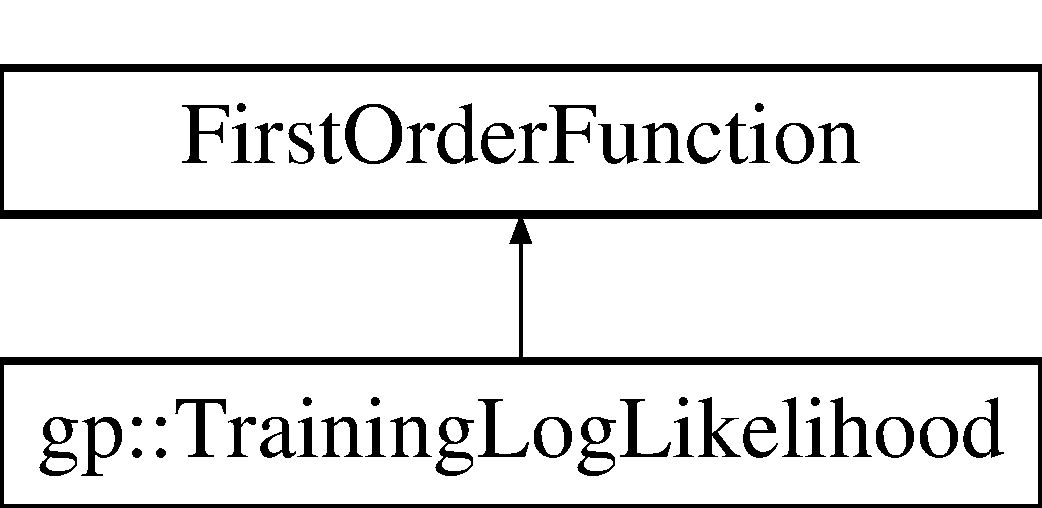
\includegraphics[height=2.000000cm]{classgp_1_1_training_log_likelihood}
\end{center}
\end{figure}
\subsection*{Public Member Functions}
\begin{DoxyCompactItemize}
\item 
\hypertarget{classgp_1_1_training_log_likelihood_a8b5d7ce6c0cb0b705cf08d063935cf2a}{}\label{classgp_1_1_training_log_likelihood_a8b5d7ce6c0cb0b705cf08d063935cf2a} 
{\bfseries Training\+Log\+Likelihood} (const Point\+Set \&points, const Vector\+Xd $\ast$targets, const Kernel\+::\+Ptr \&kernel, double noise)
\item 
\hypertarget{classgp_1_1_training_log_likelihood_a436617b7f5e4d393e1f65fc4a77c66dd}{}\label{classgp_1_1_training_log_likelihood_a436617b7f5e4d393e1f65fc4a77c66dd} 
bool {\bfseries Evaluate} (const double $\ast$const parameters, double $\ast$cost, double $\ast$gradient) const
\item 
\hypertarget{classgp_1_1_training_log_likelihood_a6a1682cbb9f44981acb7dfedc4729ffa}{}\label{classgp_1_1_training_log_likelihood_a6a1682cbb9f44981acb7dfedc4729ffa} 
int {\bfseries Num\+Parameters} () const
\end{DoxyCompactItemize}


\subsection{Detailed Description}


Definition at line 56 of file cost\+\_\+functors.\+hpp.



The documentation for this class was generated from the following file\+:\begin{DoxyCompactItemize}
\item 
/\+Users/davidfridovichkeil/\+Documents/\+Developer/gp/include/optimization/cost\+\_\+functors.\+hpp\end{DoxyCompactItemize}

%--- End generated contents ---

% Index
\backmatter
\newpage
\phantomsection
\clearemptydoublepage
\addcontentsline{toc}{chapter}{Index}
\printindex

\end{document}
